% !TEX root = ./../../_Thesis.tex

% chapter's name and label
\chapter{Anonymous Participant Data}
\label{chap:AppendixA}

This appendix contains data captured through the experiments described in Section \ref{subsec:ExperimentalDesign}. The following participant data is related to the subject with ID number 001. The complete database describing the results can be downloaded at: 

\noindent
\textbf{http://www.inf.ufrgs.br/\textasciitilde mlkrueger/MSc\_Dissertation/IPD\_Database.zip}

~

\begin{description}

	\item[ID Number]			\hfill \\
	Subject identification number
	
	\item[REF. DATA]			\hfill \\
	Examination reference data
	
	\item[EYE DROPS] 			\hfill \\
	Whether cycloplegic eye drop was used or not
	
	\item[VD]					\hfill \\
	Vertex distance configured in the TOPCON KR-8900 Autorefractor device
	
	\item[CYL]					\hfill \\
	Cylinder notation (Brazilian notation is the negative one)
	
	\item[PD] 					\hfill \\
	Pupil distance
	
	\item[S]					\hfill \\
	Spherical
	
	\item[C]					\hfill \\
	Cylindrical
	
	\item[A] 					\hfill \\
	Cylindrical axis
	
	\item[S.E.]					\hfill \\
	Spherical Equivalent ($SE = S+(C/2)$)
	
	\item[MV]					\hfill \\
	Minimum visible
	
	\item[ET] 					\hfill \\
	Elapsed time
	
	\item[LM]					\hfill \\
	Lux Mean
	
\end{description}

\begin{figure}[h]
	
	\centering
	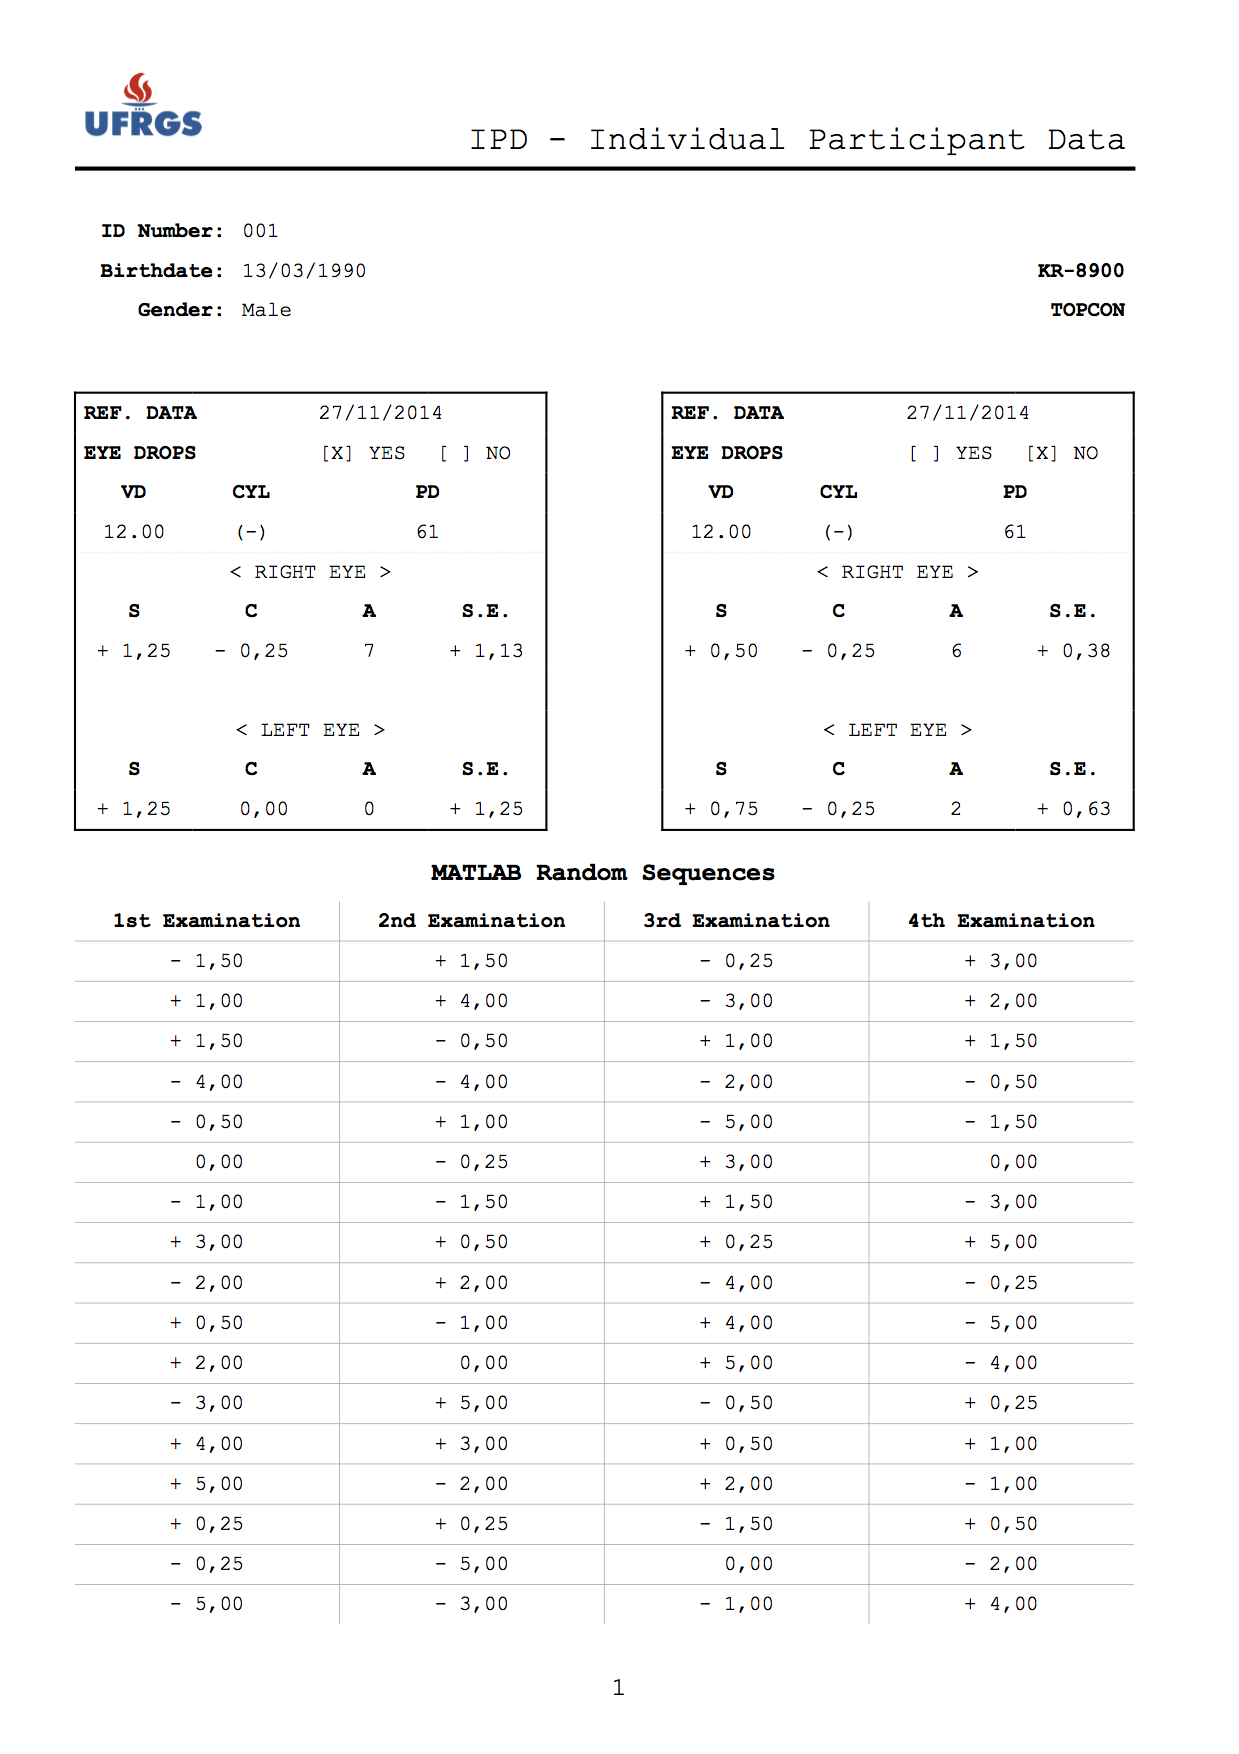
\includegraphics[width=1.0\linewidth]{__Images/08/IPD_001_1.png}
\end{figure}

\begin{figure}[h]
	
	\centering
	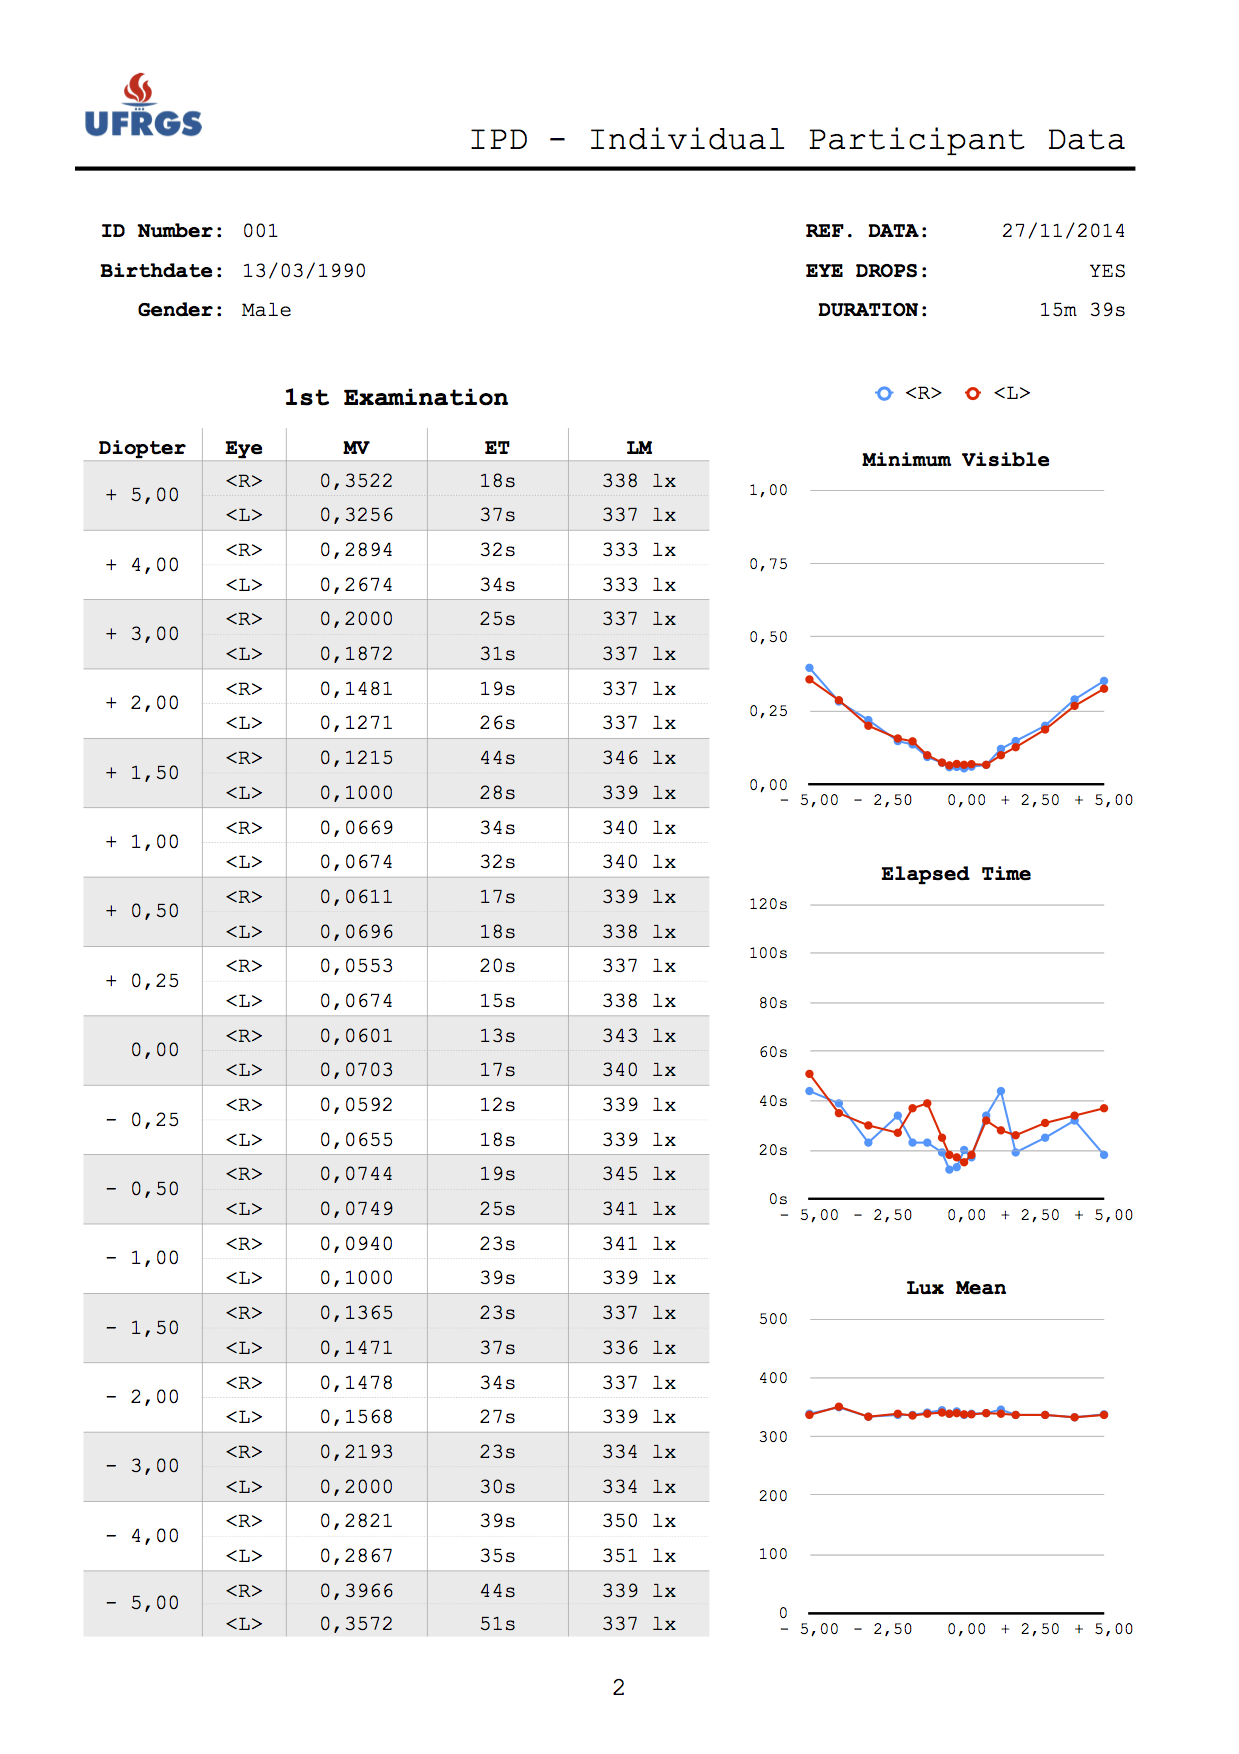
\includegraphics[width=1.0\linewidth]{__Images/08/IPD_001_2.png}
\end{figure}

\begin{figure}[h]
	
	\centering
	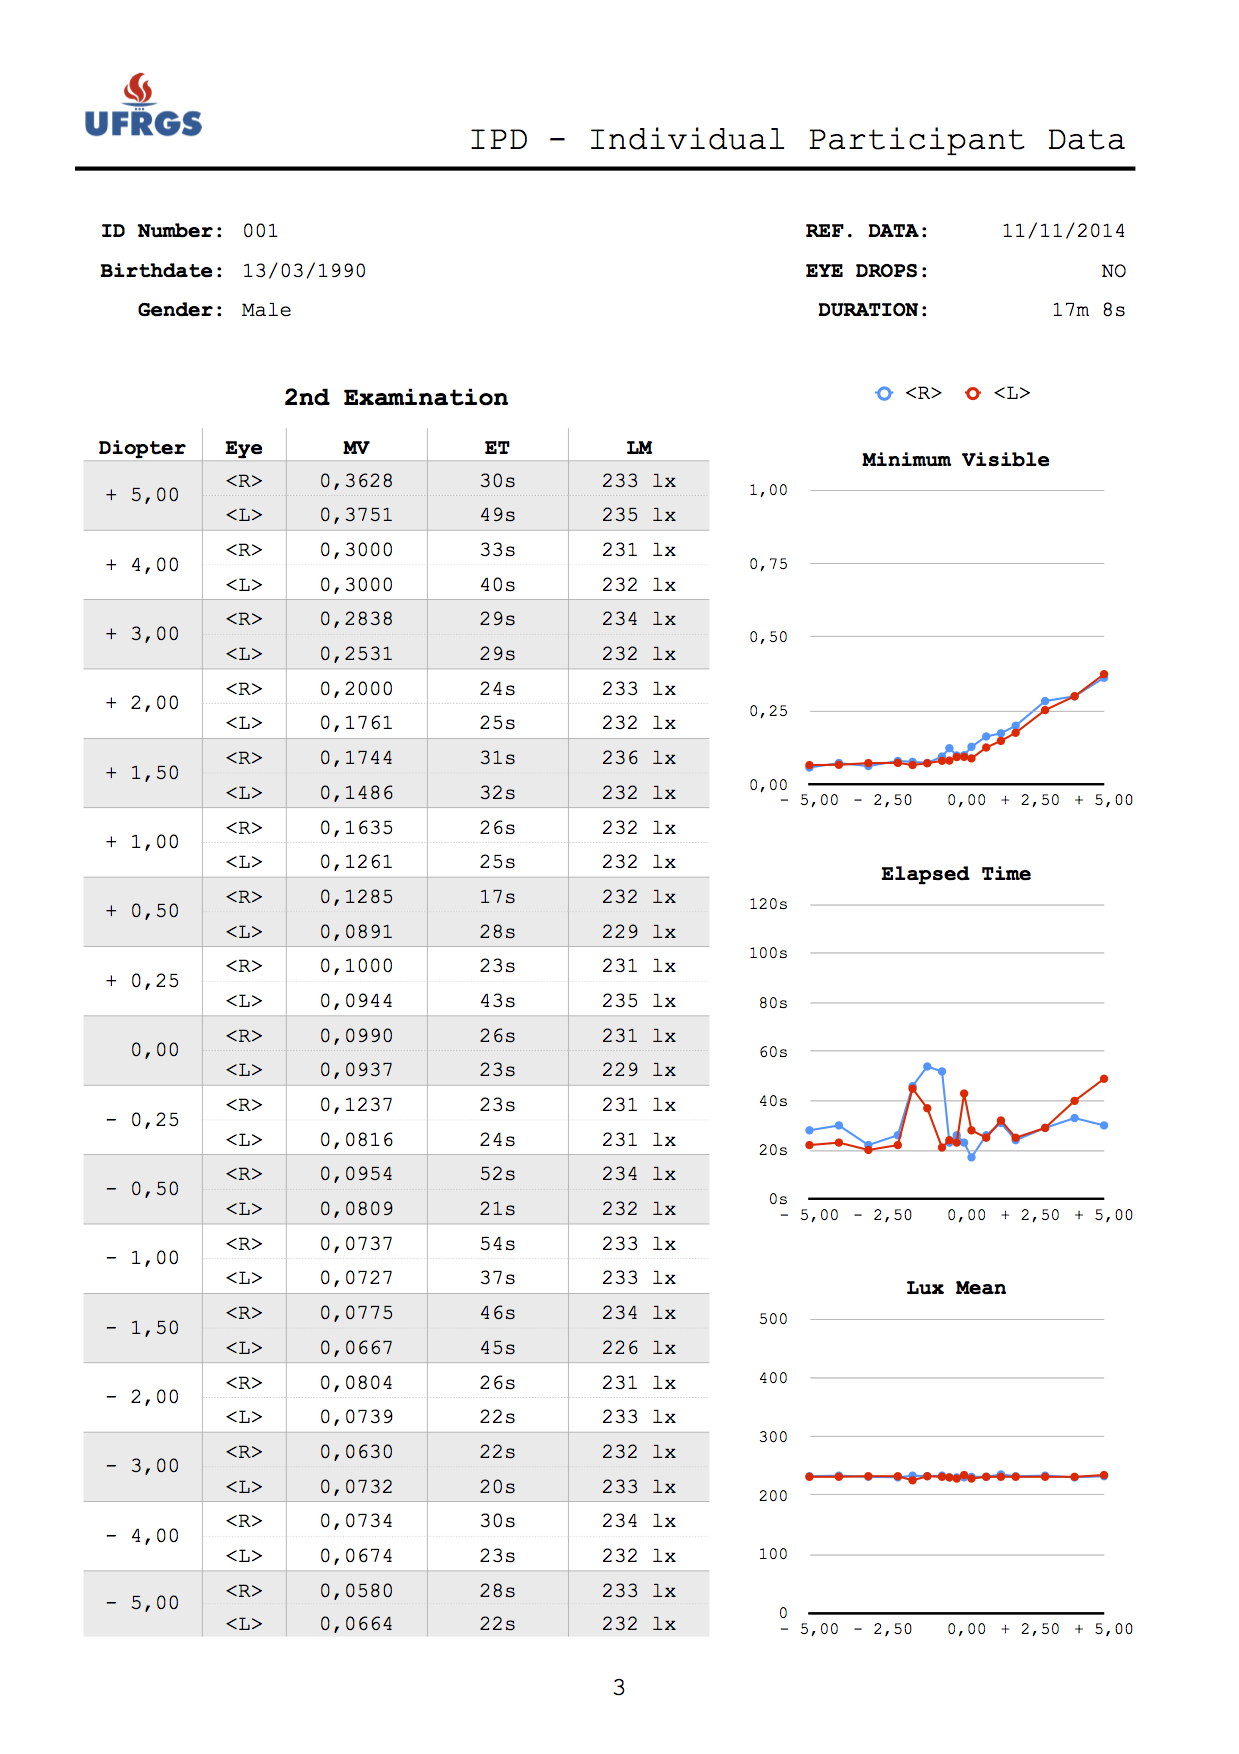
\includegraphics[width=1.0\linewidth]{__Images/08/IPD_001_3.png}
\end{figure}

\begin{figure}[h]
	
	\centering
	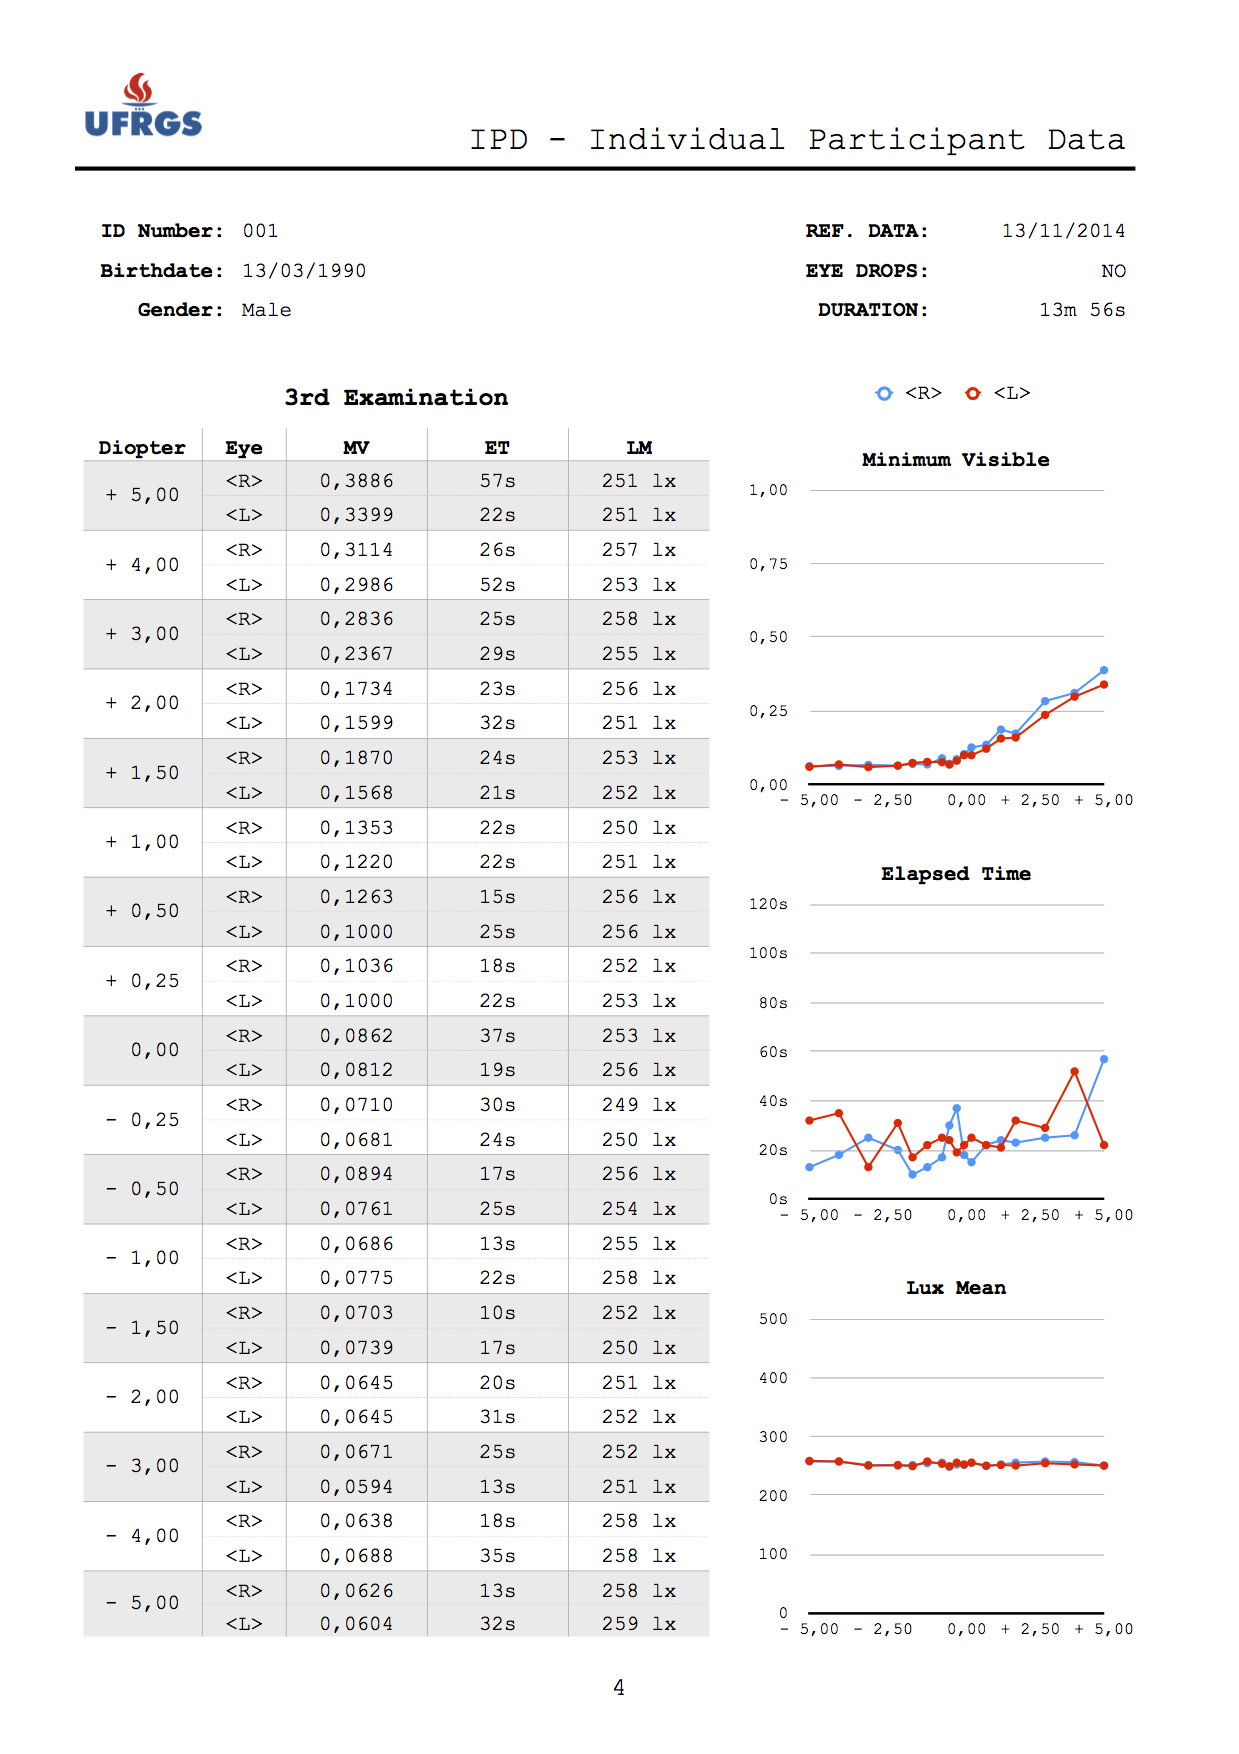
\includegraphics[width=1.0\linewidth]{__Images/08/IPD_001_4.png}
\end{figure}

\begin{figure}[h]
	
	\centering
	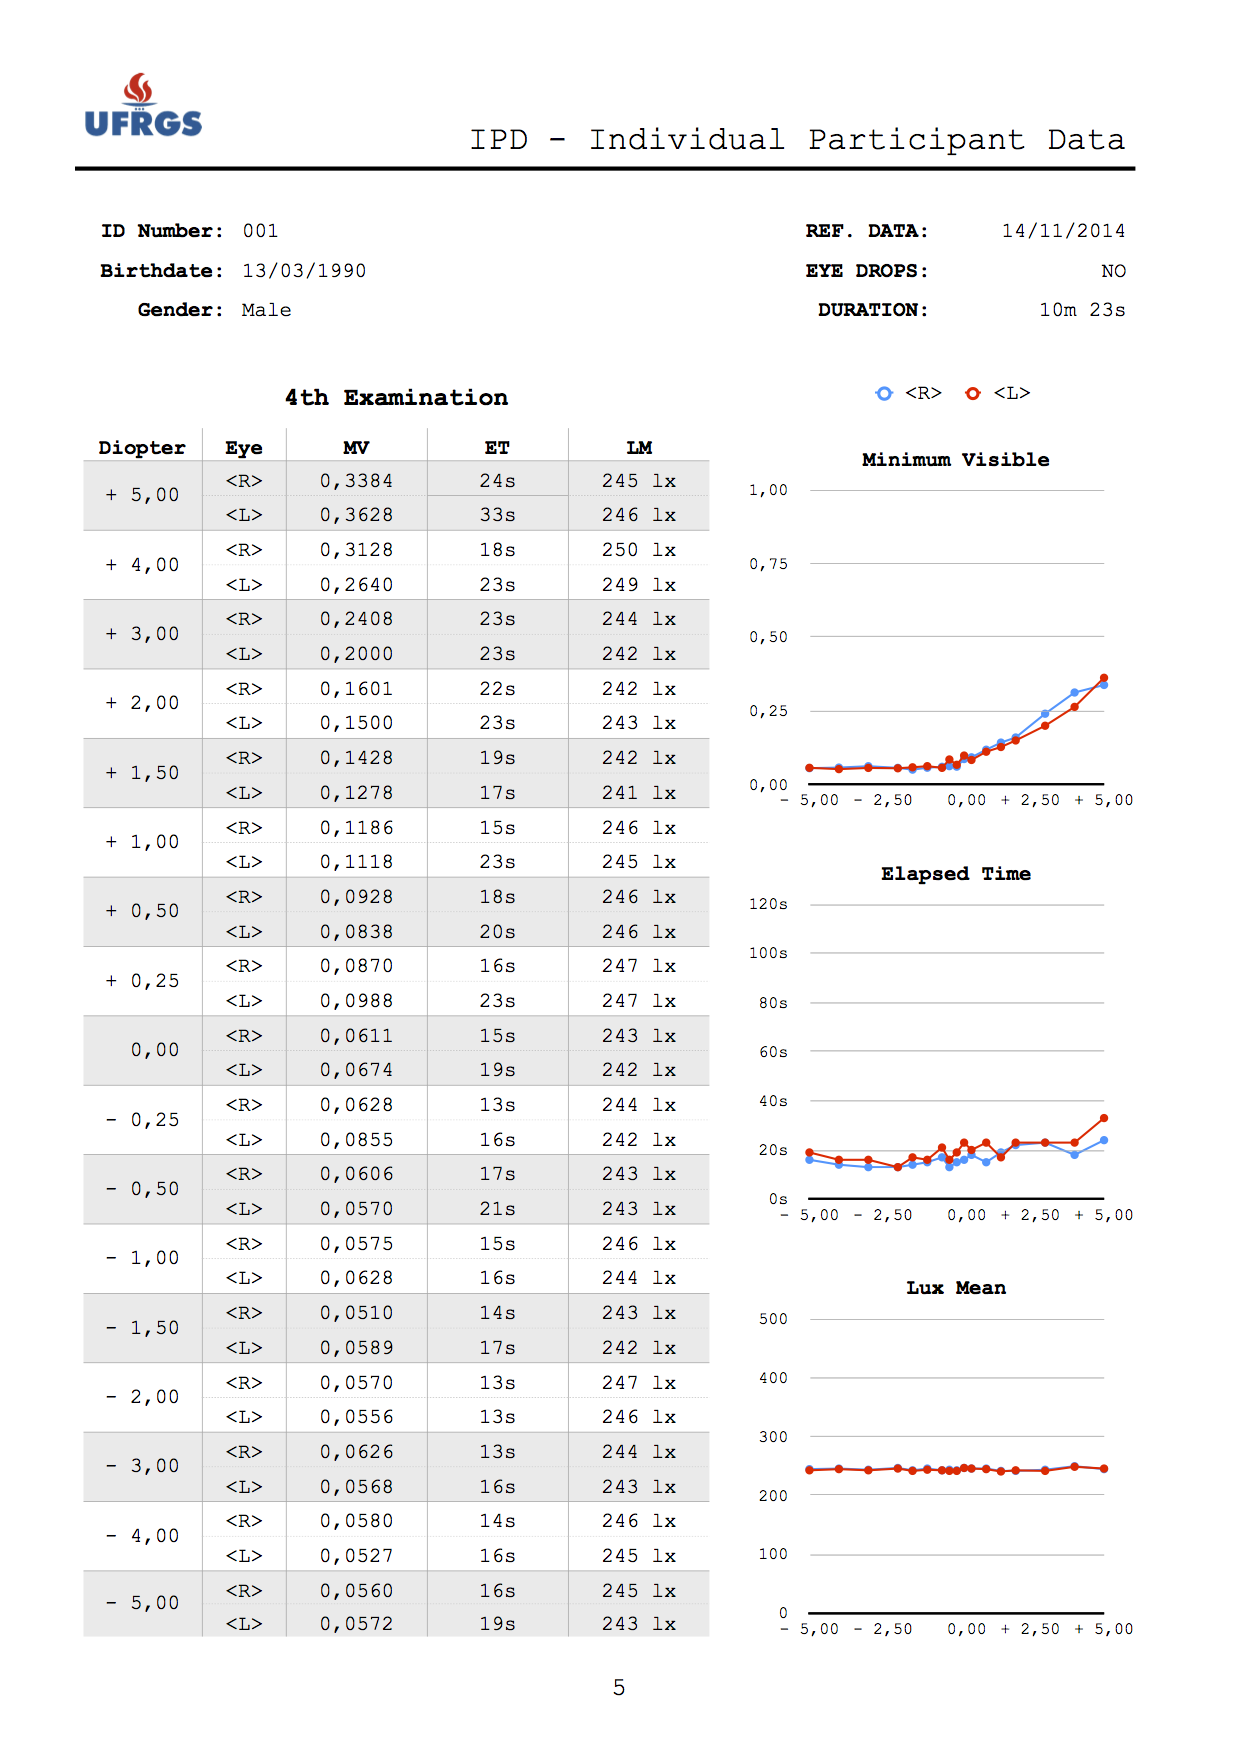
\includegraphics[width=1.0\linewidth]{__Images/08/IPD_001_5.png}
\end{figure}

\begin{figure}[h]
	
	\centering
	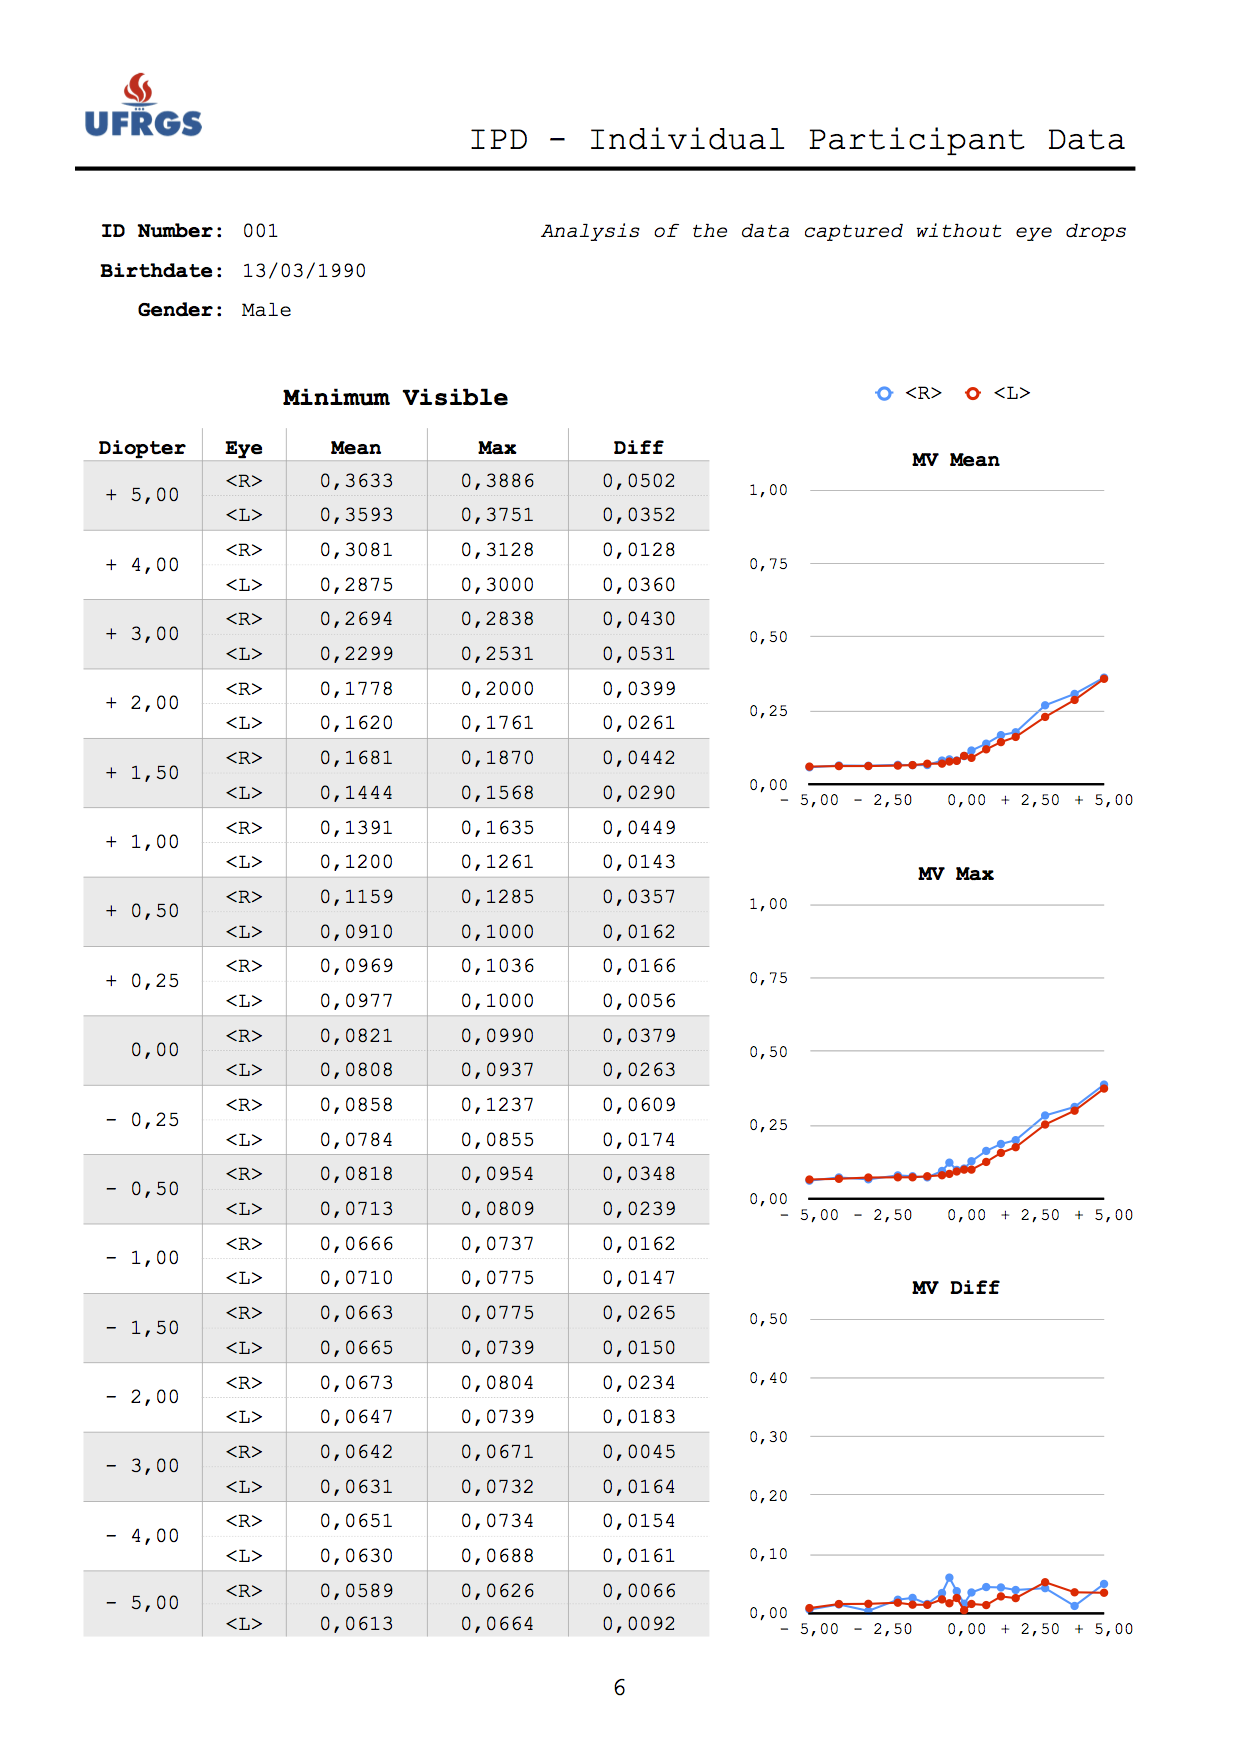
\includegraphics[width=1.0\linewidth]{__Images/08/IPD_001_6.png}
\end{figure}